\chapter{Graphics}
\label{cha:graphics}
\begin{quote}
If I could say it in words there would be no reason to paint. --- Edward Hopper
\end{quote}
\section{PyPedal Graphics}
\label{sec:graphics-overview}
\index{graphics}
\PyPedal{} is capable of producing graphics from information contained in a pedigree, including pedigree drawings, line graphs of changes in genetic diversity over time, and visualizations of numerator relationship matrices.  These graphics are non-interactive: output images are created and written to output files.  A separate program must be used to view and/or print the image; web browsers make reasonably good viewers for a small number of images.  If you are creating and viewing large numbers of images you may want to obtain an image management package for your platform.  Default and supported file formats for each of the graphics routines are presented in Table \ref{tbl:pypedal-graphics-formats}.
\begin{center}
    \tablecaption{Default graphics formats.}
    \tablefirsthead{\hline Routine & Default Format & Supported Formats \\ \hline}
    \tablehead{\hline Routine & Default Format & Supported Formats \\ \hline}
    \tabletail{\hline \multicolumn{3}{l}{\small\sl continued on next page} \\ \hline}
    \tablelasttail{\hline}
    \label{tbl:pypedal-graphics-formats}
    \begin{xtabular}{llp{2in}}
	draw\_pedigree & JPG & JPG, PNG, PS \\
	new\_draw\_pedigree & JPG & JPG, PNG, PS \\
	pcolor\_matrix\_pylab & PNG & PNG only \\
	plot\_founders\_by\_year & PNG & PNG only \\
	plot\_founders\_pct\_by\_year & PNG & PNG only \\
	plot\_line\_xy & PNG & PNG only \\
	rmuller\_pcolor\_matrix\_pil & PNG & PNG only \\
	rmuller\_spy\_matrix\_pil & PNG & PNG only \\
	spy\_matrix\_pylab & PNG & PNG only \\
    \end{xtabular}
\end{center}
\subsection{Drawing Pedigrees}
\label{sec:graphics-drawing-pedigrees}
\index{graphics!drawing pedigrees}
The pedigree from Figure 2 in Boichard et al. \citeyear{ref352} is shown in Figure \ref{fig:boichard2-pedigree}, and shows males enclosed in rectangles and females in ovals.  Figure \ref{fig:new-ids2-pedigree-basic} shows a pedigree in which strings are used for animal IDs; animal are enclosed in ovals because sexes were not specified in the pedigree file and the \member{set\_sexes} option was not specified.  A more complex German Shepherd pedigree is presented in Figure \ref{fig:doug-pedigree-basic}; the code used to create this pedigree is:
\begin{verbatim}
pyp_graphics.draw_pedigree(example, gfilename='doug_p_rl_notitle', gname=1,
    gdirec='RL', gfontsize=12)
\end{verbatim}
\begin{figure}
  \begin{center}
    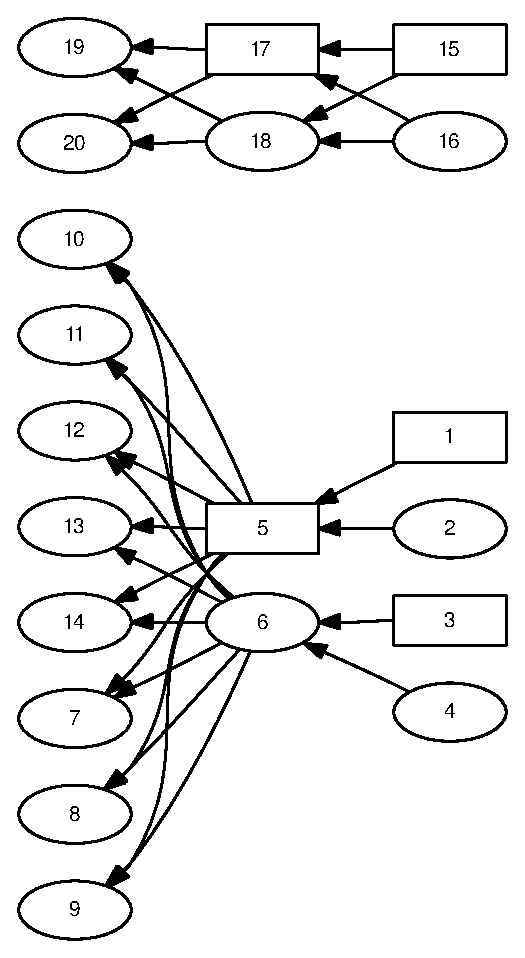
\includegraphics[width=4in]{boichard2Pedigree.eps}
    \caption{Pedigree 2 from Boichard et al. (1997)}
    \label{fig:boichard2-pedigree}
  \end{center}
\end{figure}
\begin{figure}
  \begin{center}
    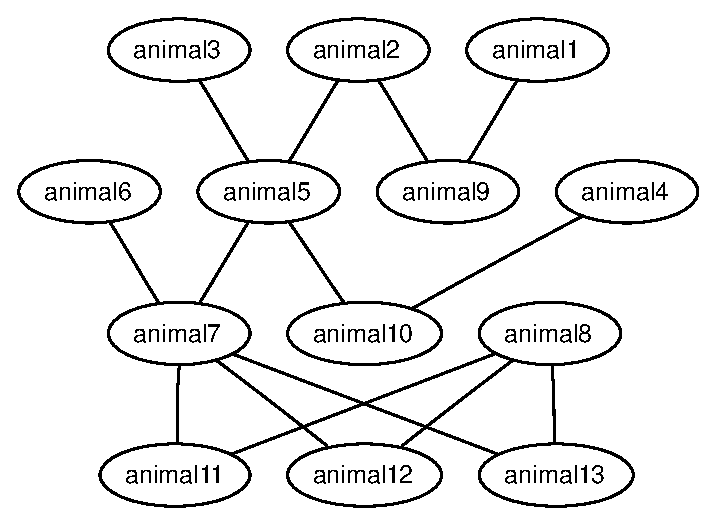
\includegraphics[width=3in]{BoichardPedigreeBasic.eps}
    \caption{A pedigree with strings as animal IDs}
    \label{fig:new-ids2-pedigree-basic}
  \end{center}
\end{figure}
\begin{figure}
  \begin{center}
    \includegraphics[width=4in]{dougPRlNotitle.eps}
    \caption{German Shepherd pedigree}
    \label{fig:doug-pedigree-basic}
  \end{center}
\end{figure}
The resulting graphic is written to doug\_p\_rl\_notitle.jpg; note from Table \ref{tbl:pypedal-graphics-formats} that the default file format for \function{draw\_pedigree()} is \textbf{JPG} rather than \textbf{PNG}, as is the case for the other graphics routines.  To get a PNG simply pass the argument \var{gformat='png'} to \function{draw\_pedigree()}.  For details on the options taken by \function{draw\_pedigree()} please refer to the API documentation (Section \ref{sec:pyp-graphics-draw-pedigree}). \function{draw\_pedigree()} uses rectangles to indicates known males, circles to indicate known females, and octagons to indicate animals of unknown sex.

Pedigrees can also be colored using the \function{color\_pedigree()} function in the \module{pyp\_jbc} module. At present, animals are shaded either by the number of sons produced or by the total number of descendants. The five-generation pedigree of the Newfoundland dog King von der D\"{u}ssel is presented in Figure \ref{fig:newfoundland-colored-pedigree} (\url{http://www.newfoundlanddog-database.net/en/ahnen.php?num=0000025330}, data used with permission), and the nodes are shaded based on number of descendants.
\begin{figure}
  \begin{center}
    \includegraphics[width=4in]{newfoundland.eps}
    \caption{Newfoundland colored pedigree}
    \label{fig:newfoundland-colored-pedigree}
  \end{center}
\end{figure}

\fixme{Windows users should set the \var{drawers} keyword to 'old' when calling \function{color\_pedigree()}. This will call \function{draw\_colored\_pedigree()} rather than \function{new\_draw\_colored\_pedigree()}. The latter requires that PyGraphviz library be installed and there is not yet an easy way to install it on Windows.}
\subsection{Drawing Line Graphs}\label{sec:graphics-drawing-line-graphs}\index{graphics!drawing line graphs}
The \texttt{plot\_line\_xy()} routine provides a convenient tool for creating two-dimensional line graphs.  Figure \ref{fig:ayrshire-coi-graph} shows the plot of inbreeding by birth year for the US Ayrshire cattle population.  The plot is produced by the call:
\begin{verbatim}
pyp_db.loadPedigreeTable(ay)
coi_by_year = pyp_reports.meanMetricBy(ay,metric='fa',byvar='by')
cby = coi_by_year
del(cby[1900])
pyp_graphics.plot_line_xy(coi_by_year, gfilename='ay_coi_by_year',
    gtitle='Inbreeding coefficients for Ayrshire cows', gxlabel='Birth year',
    gylabel='Coefficient of inbreeding')
\end{verbatim}
\begin{figure}
  \begin{center}
    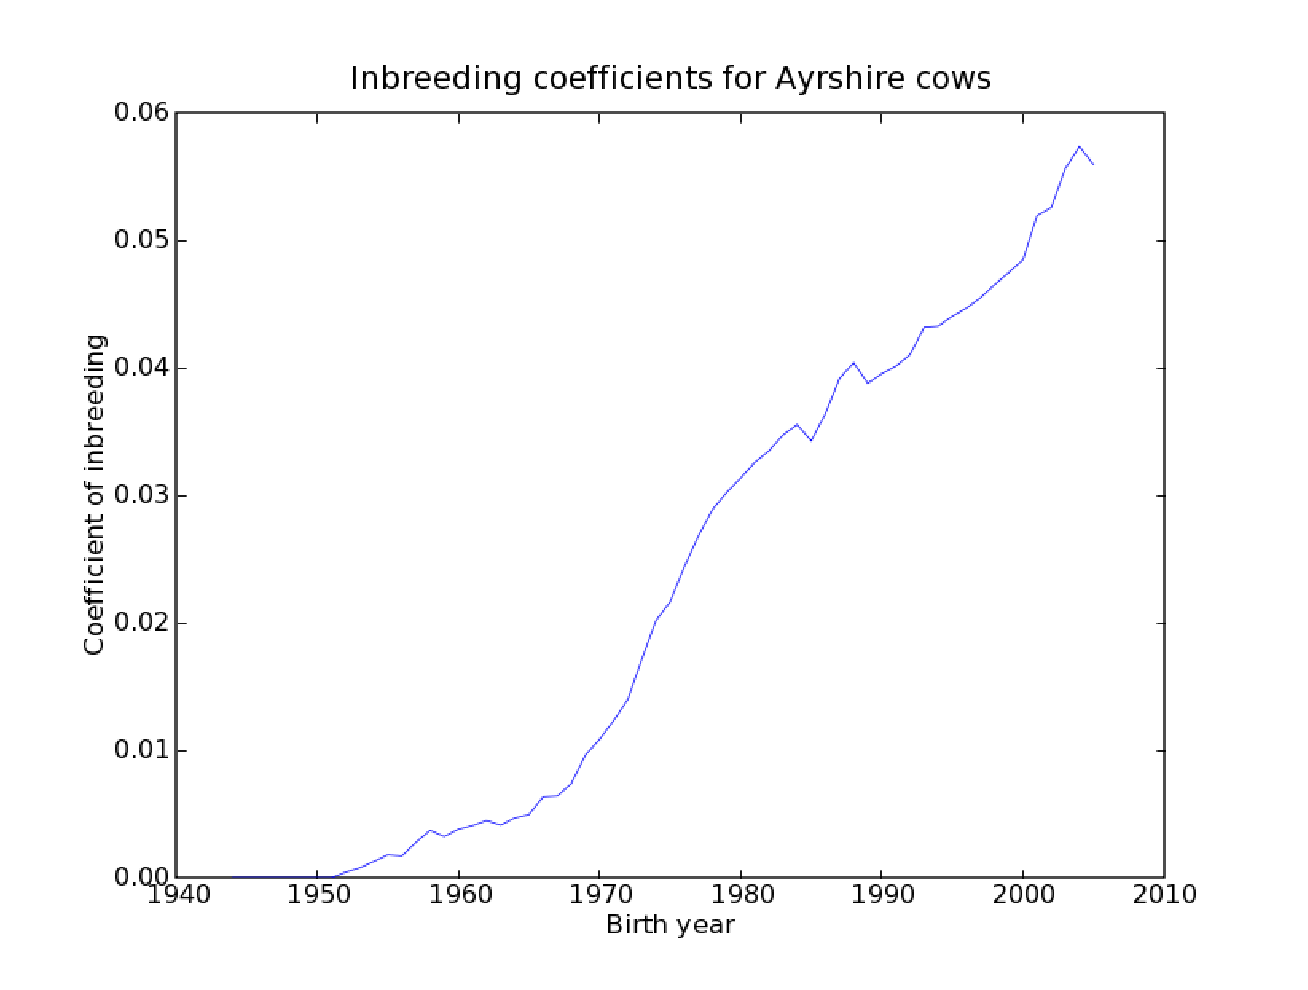
\includegraphics[width=4in]{ayCoiByYear.eps}
    \caption{Average inbreeding by birth year for the US Ayrshire cattle population}
    \label{fig:ayrshire-coi-graph}
  \end{center}
\end{figure}
The code above uses \function{pyp_reports.meanMetricBy()} (see \ref{sec:pyp-reports-mean-metric-by}) to populate \var{coi_by_year}; the keys in \var{coi\_by\_year} are plotted in the x-axis, and the values are plotted on the y-axis.  The default birth year, 1900, was deleted from the dictionary before the plot was drawn because leaving the default birthyear in the plot was distracting and somewhat misleading.  The only restriction that you have to observe is that the value plotted on the y-ais has to be a numeric quantity.

If you need more complicated plots than are produced by \function{plot\_line\_xy()} you can write a new plotting function (Chapter \ref{cha:newfeatures}) that uses the tools in matplotlib (\url{http://matplotlib.sourceforge.net/}). For complete details on the options taken by \function{plot\_line\_xy{}} please refer to the API documentation (\ref{sec:pyp-graphics-plot-line-xy}).
\subsection{Visualizing Numerator Relationship Matrices}
\label{sec:graphics-visualizing-nrm}
\index{graphics!visualizing relationship matrices}
Two routines are provided for visualization of numerator relationship matrices (NRM), \function{rmuller_pcolor_matrix_pil()} and \function{rmuller_spy_matrix_pil()}.

As an example, we will consider the NRM for the pedigree in Figure \ref{fig:boichard2-pedigree}.  The matrix is square and symmetric; the diagonal values correspond to $1+f_a$, where $f_a$ is an animal's coefficient of inbreeding; animals with a diagonal element $>1$ are inbred.
\[
    \scriptsize
    \left[ \begin{array}{llllllllllllllllllll}
        1. & 0. & 0. & 0. & 0.5 & 0. & 0.25 & 0.25 & 0.25 & 0.25 & 0.25 & 0.25 & 0.25 & 0.25 & 0. & 0. & 0. & 0. & 0. & 0. \\
        0. & 1. & 0. & 0. & 0.5 & 0. & 0.25 & 0.25 & 0.25 & 0.25 & 0.25 & 0.25 & 0.25 & 0.25 & 0. & 0. & 0. & 0. & 0. & 0. \\
        0. & 0. & 1. & 0. & 0.  & 0.5 & 0.25 & 0.25 & 0.25 & 0.25 & 0.25 & 0.25 & 0.25 & 0.25 & 0. & 0. & 0. & 0. & 0. & 0. \\
        0. & 0. & 0. & 1. & 0. & 0.5 & 0.25 & 0.25 & 0.25 & 0.25 & 0.25 & 0.25 & 0.25 & 0.25 & 0. & 0. & 0. & 0. & 0. & 0. \\
        0.5 & 0.5 & 0. & 0. & 1. & 0. & 0.5 & 0.5 & 0.5 & 0.5 & 0.5 & 0.5 & 0.5 & 0.5 & 0. & 0. & 0. & 0. & 0. & 0. \\
        0. & 0. & 0.5 & 0.5 & 0. & 1. & 0.5 & 0.5 & 0.5 & 0.5 & 0.5 & 0.5 & 0.5 & 0.5 & 0. & 0. & 0. & 0. & 0. & 0. \\
        0.25 & 0.25 & 0.25 & 0.25 & 0.5 & 0.5 & 1. & 0.5 & 0.5 & 0.5 & 0.5 & 0.5 & 0.5 & 0.5 & 0. & 0. & 0. & 0. & 0. & 0. \\
        0.25 & 0.25 & 0.25 & 0.25 & 0.5 & 0.5 & 0.5 & 1. & 0.5 & 0.5 & 0.5 & 0.5 & 0.5 & 0.5 & 0. & 0. & 0. & 0. & 0. & 0. \\
        0.25 & 0.25 & 0.25 & 0.25 & 0.5 & 0.5 & 0.5 & 0.5 & 1. & 0.5 & 0.5 & 0.5 & 0.5 & 0.5 & 0. & 0. & 0. & 0. & 0. & 0. \\
        0.25 & 0.25 & 0.25 & 0.25 & 0.5 & 0.5 & 0.5 & 0.5 & 0.5 & 1. & 0.5 & 0.5 & 0.5 & 0.5 & 0. & 0. & 0. & 0. & 0. & 0. \\
        0.25 & 0.25 & 0.25 & 0.25 & 0.5 & 0.5 & 0.5 & 0.5 & 0.5 & 0.5 & 1. & 0.5 & 0.5 & 0.5 & 0. & 0. & 0. & 0. & 0. & 0. \\
        0.25 & 0.25 & 0.25 & 0.25 & 0.5 & 0.5 & 0.5 & 0.5 & 0.5 & 0.5 & 0.5 & 1. & 0.5 & 0.5 & 0. & 0. & 0. & 0. & 0. & 0. \\
        0.25 & 0.25 & 0.25 & 0.25 & 0.5 & 0.5 & 0.5 & 0.5 & 0.5 & 0.5 & 0.5 & 0.5 & 1. & 0.5 & 0. & 0. & 0. & 0. & 0. & 0. \\
        0.25 & 0.25 & 0.25 & 0.25 & 0.5 & 0.5 & 0.5 & 0.5 & 0.5 & 0.5 & 0.5 & 0.5 & 0.5 & 1. & 0. & 0. & 0. & 0. & 0. & 0. \\
        0. & 0. & 0. & 0. & 0. & 0. & 0. & 0. & 0. & 0. & 0. & 0. & 0. & 0. & 1. & 0. & 0.5 & 0.5 & 0.5 & 0.5 \\
        0. & 0. & 0. & 0. & 0. & 0. & 0. & 0. & 0. & 0. & 0. & 0. & 0. & 0. & 0. & 1. & 0.5 & 0.5 & 0.5 & 0.5 \\
        0. & 0. & 0. & 0. & 0. & 0. & 0. & 0. & 0. & 0. & 0. & 0. & 0. & 0. & 0.5 & 0.5 & 1. & 0.5 & 0.75 & 0.75 \\
        0. & 0. & 0. & 0. & 0. & 0. & 0. & 0. & 0. & 0. & 0. & 0. & 0. & 0. & 0.5 & 0.5 & 0.5 & 1. & 0.75 & 0.75 \\
        0. & 0. & 0. & 0. & 0. & 0. & 0. & 0. & 0. & 0. & 0. & 0. & 0. & 0. & 0.5 & 0.5 & 0.75 & 0.75 & 1.25 & 0.75 \\
        0. & 0. & 0. & 0. & 0. & 0. & 0. & 0. & 0. & 0. & 0. & 0. & 0. & 0. & 0.5 & 0.5 & 0.75 & 0.75 & 0.75 & 1.25
    \end{array} \right]
    \normalsize
\]
Note that the array only contains six distinct values: 0., 0.25, 0.5, 0.75, 1.0, and 1.25.  These six values will be used to create the color map used by \function{rmuller_pcolor_matrix_pil()}.

\function{rmuller_pcolor_matrix_pil()} produces pseudocolor plots from NRM.  A pseudocolor plot is an array of cells that are colored based on the values the corresponding cells in the NRM. The minimum and maximum values in the NRM are assigned the first and last colors in the colormap; other cells are colored by mapping their values to colormap elements.  In the example above, the minimum value is 0.0 and the maximum value is 1.0 (Figure \ref{fig:boichard2-pseudocolor}).  The two inbred animals in the population are easily identified as the yellow diagonal elements in the bottom-left corner of the matrix.
\begin{figure}[tb]
  \begin{center}
    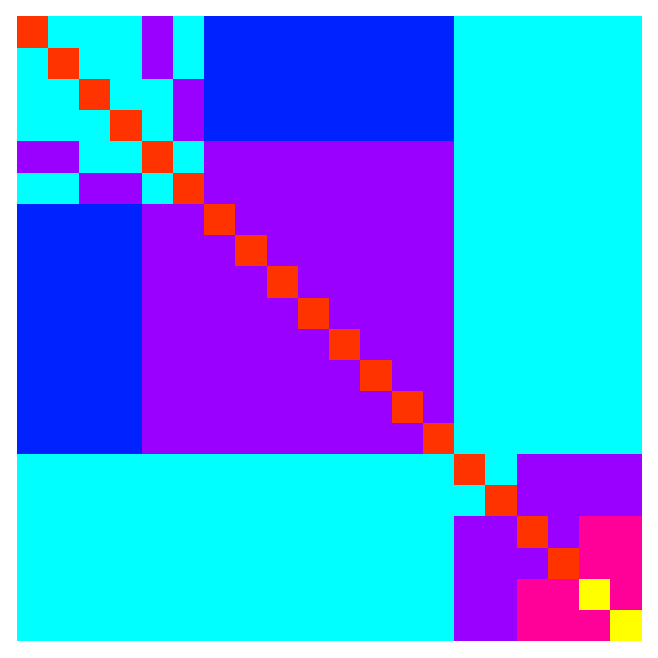
\includegraphics[width=3in]{boichard2Pcolor.eps}
    \caption{Pseudocolored NRM from the Boichard et al. (1997) pedigree}
    \label{fig:boichard2-pseudocolor}
  \end{center}
\end{figure}
\function{rmuller_spy_matrix_pil()} is similar to \function{rmuller_pcolor_matrix_pil()}, but it is used to visualize the sparsity of a matrix.  Cells are either filled, indicating that the value is non-zero, or not filled, indicating that the cell's value is zero.  In Figure \ref{fig:boichard2-sparsity} it is easy to see the two separate families in the pedigree.
\begin{figure}[tb]
  \begin{center}
    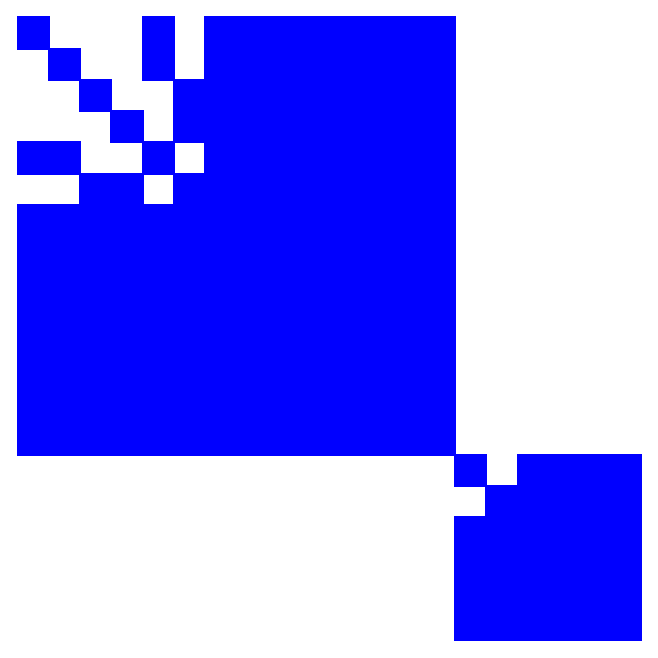
\includegraphics[width=3in]{boichard2Spy.eps}
    \caption{Sparsity of the NRM from the Boichard et al. (1997) pedigree}
    \label{fig:boichard2-sparsity}
  \end{center}
\end{figure}